\subsection{``Hello World!''}
We first try writing a simple macro that prints ''Hello World!'' in the log window of ImageJ. 

To open the macro editor, select \ijmenu{[PlugIns -> New -> Macro]} from the menu.  
This will create a new window where you can write macro (we call this ''macro
editor'', fig\ref{fig_MacroEditor}).

\begin{indentFiji}
In Fiji you could use more advanced interface called ''script editor'' 
by \ijmenu{[File -> New -> Script]}. It should look like \ref{fig_ScriptEditor}.
In the script editor, you already see a blank text field where you could write a macro. 
From script editor's own menu, select \ijmenu{[Language -> IJ1 Macro]}. 
By sepcifying the language, syntax highlighter turns on to do automatic coloring of ImageJ functions.\footnote{The macro editor (also the Fiji script editor) has simple debugger function. Debugger assists you to correct mistakes in the code. 
This is convenient when the code becomes long. 
Macro can be written in any text editor such as "Notepad" in Windows but of course 
there is no debugger function available in this case.}.  
\end{indentFiji}

Later when you want to start writing another new macro, just generate a new tab by \ijmenu{[File > New]} and then select \ijmenu{[Language -> ImageJ Macro]} again.

Then write your first macro as shown below. In the second line DON'T forget to
indent the line using tab or spaces\footnote{In ImageJ macro, indenting is not a required
syntax for writing macros but doing this will be very very helpful afterward. You
will understand it as the macro you write becomes longer}. Omit the line
numbers! These numbers were added just for explanation.

%Code 1
%\begin{lstlisting}
%macro "print_out" {
%	print("Hello World!");
%}
%\end{lstlisting}
\lstinputlisting{code/code01.ijm}
%\lstinputlisting[language=Java]{code/code01.ijm}


\begin{figure}[htbp]
\begin{center}
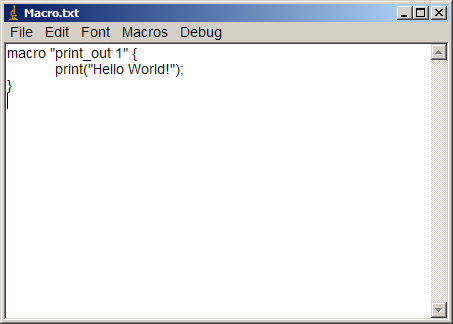
\includegraphics[scale=0.6]{fig/editor_helloworld_IJ.png}
\caption{Macro Editor of ImageJ} \label{fig_MacroEditor}
\end{center}
\end{figure}

\begin{figure}[hbtp]
\begin{center}
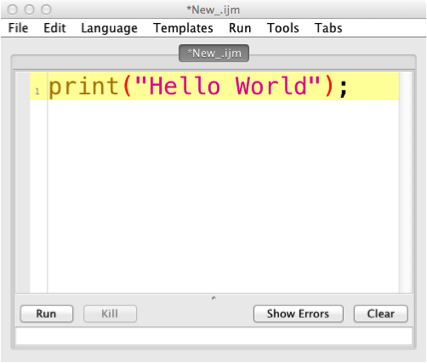
\includegraphics[scale=1.0]{fig/editor_helloworld_singleline.png}
\caption{Script Editor of the Fiji distribution} \label{fig_ScriptEditor}
\end{center}
\end{figure}

From the macro editor menu, running the code by \ijmenu{[Macros->
Run Macro]}\footnote{"Macros" in the menu appears only when the macro editing
window is active}. You could also run the code by shortcut keys (Windows:
ctrl-r, OSX command-r) as well. 
 
\begin{indentFiji}
Fiji:  Use \ijmenu{[Run -> Run]} from the script editor menu. Shortcut keys are
same as in ImageJ. You could also use ``run'' button in the script editor. 
\end{indentFiji}
This will create a new window "Log". Within the log window, "Hello World" will
be printed.

\begin{figure}[hbtp]
\begin{center}
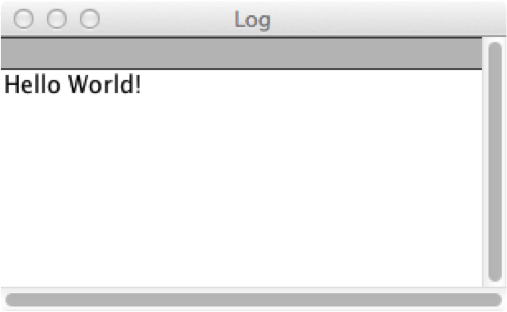
\includegraphics[scale=1.0]{fig/helloworld_logwindow.png}
\caption{Hello World Output} \label{fig_HelloWorldLog}
\end{center}
\end{figure}

Explanation for the Code 1:\\
\begin{itemize}
\item line 1: You are declaring that a macro code starts and the code is contained between 
curly braces \{\}. "print\_out" will be the name of macro. 

\item line2: print() function orders ImageJ to print out the content within the parenthesis 
in the "Log" window. The text to be printed must be contained within the double quotes (""). 
The best reference for ImageJ macro functions is in the ImageJ web site
\footnote{\url{http://rsbweb.nih.gov/ij/developer/macro/functions.html}}. 
For example, you could find definition of print("") function on the web site as quoted below:\\
%\item
\begin{indentCom}
%\begin{minipage}[c][18em][c]{0.85\textwidth}
\fbox{
\parbox[b][20em][c]{0.80\textwidth}{
\textbf{print(string)}\\
Outputs a string to the "Log" window. Numeric arguments are automatically converted to strings. 
The print() function accepts multiple arguments. For example, you can use print(x,y,width, height) 
instead of print(x+" "+y+" "+width+" "+height). 
If the first argument is a file handle returned by File.open(path), 
then the second is saved in the referred file (see SaveTextFileDemo).

Numeric expressions are automatically converted to strings using four decimal places, 
or use the \ilcom{d2s} function to specify the decimal places. 
For example, print(2/3) outputs "0.6667" but print(d2s(2/3,1)) outputs "0.7".
}
}
\end{indentCom}

\item line 3: a brace tells ImageJ that the code "print\_out" finishes at this line.  
\end{itemize}
So that was the very basic of how you use a macro. To integrate the macro into the ImageJ Menu bar, 
the macro must be "installed". To do so, in the editor menu, \ijmenu{[Macros -> Install Macros]} 
\begin{indentFiji}
Fiji: [Run -> Install Macro]).
\end{indentFiji}
Check IJ menu \ijmenu{[Macros -> ]} to see that the macro is now in the menu.\\


\begin{figure}[htbp]
\begin{center}
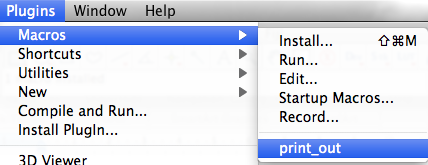
\includegraphics[scale=0.6]{fig/firstMacroInMenu.png}
\caption{Macro Now in ImageJ menu} \label{fig_MacroInMenu}
\end{center}
\end{figure}

Macro can be saved as a file and can be directly installed also. 
In the editor, do \ijmenu{[File -> Save]}. Saving dialogue window appears, 
and just save the file wherever you can remember afterwards . 
To install the macro, do \ijmenu{[PlugIns -> Macro -> Install\ldots]} 
Select the macro file you want to install.\\

%\begin{indentexercise}{1cm}
\begin{indentexercise}{1}
\item Add another line \texttt{"print("\textbackslash{}\textbackslash{}Clear");"} 
after the second line (below, code 1.5. don't forget the semi-colon at the end!). 
\item \lstinputlisting{code/code01_5.ijm}
Then test also another macro when you insert the same function in the third line (code 1.75). 
What happened?  
\item \lstinputlisting{code/code01_75.ijm}
\end{indentexercise}

\begin{indentexercise}{2}
\item Try modifying the third line in code 1.5 
and check that the modified text will be printed in the "Log" window. \\
\end{indentexercise}

\begin{indentexercise}{3}
\item Multiple macros can exist in a single file. We call this \textbf{"macro sets"}. 
Duplicate the code you wrote by copying and pasting it under the first macro. 
The second macro should have a different name. In the example shown in fig.
\ref{fig_MacroSetInMenu}, the second macro is named "pirnt\_out2".
\end{indentexercise}

\begin{figure}[h!]
\begin{center}
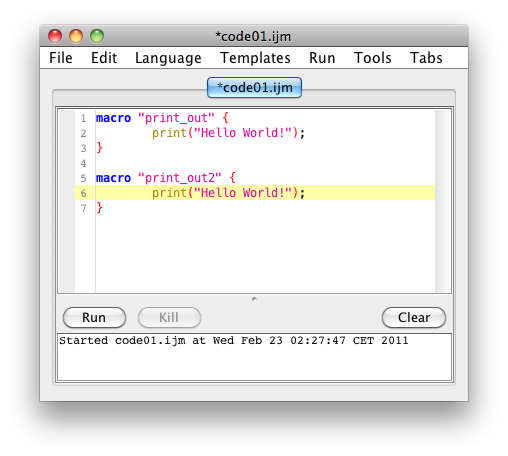
\includegraphics[scale=0.6]{fig/editor_MacroSet.png}
\caption{Macro Set} \label{fig_MacroSetInMenu}
\end{center}
\end{figure}
When macro is properly declared in this way, you could install the macro to have it as a menu item. To do so, in the editor menu select: 
\begin{indentFiji}
[Run -> Install Macro]).
\end{indentFiji}
In the main menu you should no be able to see the macro names under \ijmenu{[Plugins > Macros > ]}.

